% =========================
% CHAPTER 2 (REVISED)
% =========================
\chapter{Background of the Study}
\label{chap:background}

% ---------------------------------------------------------
\section{AI-Assisted Programming}
\label{sec:bg-ai}

Building on the terminology consolidated in Table~\ref{tab:key-definitions}, \emph{\gls{ai}-assisted programming} refers to \gls{ml}-based tools that participate in one or more stages of software development within an \gls{ide}, for instance, understanding requirements, writing or modifying code, running tests, or debugging failures \parencite{ziegler2024measuring, chen2021codex}. The scope deliberately excludes standalone model evaluations and benchmark-only settings; the focus is on assistance as it unfolds during real coding work as an interaction between a human developer and an \gls{ai} system \parencite{ziegler2024measuring}.

In practice, contemporary assistants cluster into three broad interaction types. \emph{Code completion} tools predict tokens or lines inline as developers type, offering suggestions that can be accepted, edited, or dismissed \parencite[pp.~2--3]{chen2021codex}. \emph{Chat-based assistants} provide a dialog-based interface in which developers ask natural-language questions and receive explanations, snippets, or refactoring proposals \parencite[p.~492]{ross2023programmer}. \emph{Agentic assistants} extend this by planning and executing multi-step changes, potentially across multiple files and tool calls while surfacing actions for human approval at checkpoints \parencite{vscodeCopilotAgentMode}. These types differ not only in UI but also in how initiative and responsibility are split between the system and the developer.

All three are commonly powered by \glspl{llm} (defined in Table~\ref{tab:key-definitions}). Benchmark performance illustrates capability but does not guarantee correctness in situ: Codex, for example, solved 28.8\% of HumanEval problems in a single attempt and 72.3\% with repeated sampling \parencite[p.~1]{chen2021codex}. In real IDE work, however, outputs remain \emph{probabilistic rather than verified}. This gap matters because developer time is often shifted from writing to \emph{understanding, verifying, and repairing} generated code, costs that can be substantial and are easy to miss if evaluation focuses only on generation speed \parencite{vaithilingam2022expectation, mozannar2024reading}.

A useful lens for differentiating assistance types is \emph{autonomy} in human--\gls{ai} systems. Parasuraman, Sheridan, and Wickens distinguish (1) \emph{types of automation} information \emph{acquisition}, \emph{analysis}, \emph{decision}, and \emph{action} and (2) the \emph{level} at which automation is applied, ranging from low (manual) to high (full automation) \parencite{parasuraman2000model}. For \gls{ai}-assisted programming, this implies autonomy is not a single fixed tool property: a system may strongly automate analysis (e.g., diagnosing a failing test) while keeping actions (e.g., applying edits or executing commands) gated behind explicit developer approval. This partition is central for this thesis because interaction paradigms can shift the developer role from \emph{implementer} toward \emph{supervisor}, changing where effort is spent (prompting vs review), what breaks flow, and what kinds of errors are likely to slip through \parencite{parasuraman2000model, sarkar2025codewithme}.
\linebreak
\begin{figure}[H]

  \centering

  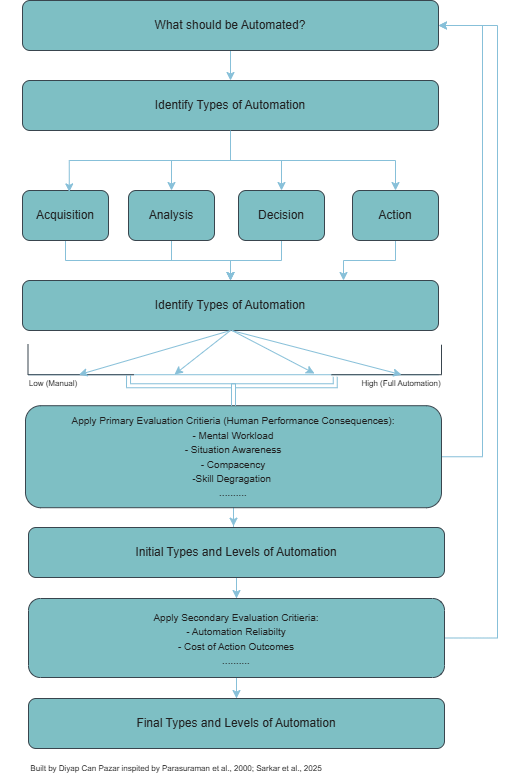
\includegraphics[width=0.60\textwidth]{figures/automation-level.png}

  \caption[Applying types and levels of automation]{Flow chart showing application of the Parasuraman et al.\ model of types and levels of automation. For each automation type (acquisition, analysis, decision, action), a level between low (manual) and high (full automation) is selected and progressively adjusted using primary human-performance consequences and secondary evaluative criteria \parencite{parasuraman2000model}.}

  \label{fig:autonomy-spectrum}

\end{figure}

The primary implication for coding tools is not simply that ``more autonomy is better,'' but that autonomy choices trade off human performance consequences. Parasuraman et al.\ emphasize evaluative criteria such as mental workload, situation awareness, complacency, and skill degradation, alongside reliability and the cost of erroneous actions \parencite{parasuraman2000model}. In an IDE setting, this translates into a concrete tension: higher autonomy can reduce interaction cost (fewer step-by-step exchanges) while increasing the \emph{supervision and verification burden} (larger diffs, fewer intermediate states, higher recovery cost when something drifts).

Despite strong capability, \glspl{llm} display systematic \emph{model-side failure modes}. These include producing code that compiles but violates intended semantics, hallucinating non-existent functions or APIs, and failing to preserve consistency across longer contexts or multi-file edits \parencite{ji2023hallucination, zhang2023sirenssong}. Security risks are particularly salient: AI assistance can raise vulnerability incidence even while developers indicate greater confidence \parencite{perry2023insecure}. Industry-focused evaluations similarly report elevated duplication, inconsistent style, and insufficient error handling in generated code, exposing a gap between ``passes tests'' and production-quality expectations \parencite{qodo2025codequality}.

Equally important are \emph{human-side failure modes}. Prior work documents over-trust and shallow verification strategies in AI-assisted programming, ranging from cursory scanning to more systematic review depending on task stakes and developer experience \parencite{barke2023trust}. More broadly, automation bias deferring to an automated recommendation even when contradictory evidence exists, is a well-established phenomenon in human factors research and transfers directly to coding workflows when outputs appear fluent and plausible \parencite{leeSee2004trust}. These risks are amplified when interaction schemes fragment attention, because interruptions and resumption costs can degrade deliberate reasoning during review \parencite{parnin2011resumption, abad2018taskInterruption}.

Together, these model-side and human-side dynamics motivate the thesis's focus on \emph{verification and visibility}. In many development contexts, the developer is the primary verification mechanism. If intermediate reasoning is hidden, diffs are large, or review time is squeezed by interaction friction, errors can propagate quietly into the codebase. This makes it essential to examine not only whether assistance accelerates tasks, but how different interaction paradigms reshape oversight capacity, workflow stability, and trust calibration \parencite{mozannar2024reading, leeSee2004trust}.

% ---------------------------------------------------------
\section{Vibe Coding as an Interaction Paradigm}
\label{sec:bg-vibe}

\emph{Vibe Coding}, operationalized in this study through GitHub Copilot's Ask mode, is an interaction paradigm in which the developer and the \gls{ai} engage in a turn-by-turn conversational exchange. The developer submits a natural-language prompt describing a desired change, the AI returns a proposed response (e.g., code snippet, explanation, refactoring suggestion), and the developer decides whether and how to integrate it before formulating the next prompt. Each exchange constitutes one interaction cycle; completing a task typically requires multiple cycles. The developer remains the primary agent throughout: deciding what to ask, when to ask, what to apply, and when to move on \parencite[pp.~85--88]{barke2023groundedcopilot}.

Under this paradigm, the human retains direct control over several important dimensions. The developer chooses the scope and specificity of prompts, selects which parts of a response to use, performs integration manually, and initiates test runs. The system does not autonomously modify files or execute commands; every change passes through deliberate developer action. In autonomy terms, this corresponds to lower levels where the system proposes and the human decides and acts \parencite[p.~287]{parasuraman2000model}.

Empirical studies of conversational \gls{ai} tools highlight recurring interaction trends. Barke, James, and Polikarpova describe \emph{acceleration} (speeding up known work) and \emph{exploration} (traversing unfamiliar territory) as two main modes \parencite[pp.~89--95]{barke2023groundedcopilot}. In both, developers iterate: clarifying requirements, refining prompts, and correcting misunderstandings. The practical strength of Vibe Coding is that it preserves high translucency and fine-grained steering: developers see the solution evolve step by step, evaluate increments in isolation, and redirect quickly when outputs drift, supporting continuous trust calibration \parencite{leeSee2004trust}.

The weakness is that this conversational overhead can accumulate across many cycles. When an initial response is incomplete or misleading, developers may enter repeated prompt-and-repair loops, fragmenting workflow and consuming time. Controlled evaluations report that debugging and understanding AI-generated code can offset expected productivity gains in chat-like usage, particularly when verification becomes the bottleneck \parencite{vaithilingam2022expectation, mozannar2024reading}.

% ---------------------------------------------------------
\section{Agentic Coding as an Interaction Paradigm}
\label{sec:bg-agentic}

\emph{Agentic Coding}, operationalized in this study through GitHub Copilot’s Agent mode, is an interaction paradigm in which the developer delegates a goal to an \gls{ai} agent that plans and executes a multi-step sequence to achieve that goal. A common workflow follows a \emph{goal → plan → act → propose → approve} structure: the developer specifies a high-level objective, the agent decomposes it, executes actions (e.g., editing multiple files, running terminal commands, iterating on failing tests), and then surfaces a consolidated result for developer review \parencite{vscodeCopilotAgentMode, sarkar2025codewithme}.

Agent mode goes beyond conversational assistance by combining multi-file context with tool-mediated actions. It is able to navigate and modify several files, invoke shell commands (e.g., running \texttt{pytest}), create new files, and iterate in response to execution feedback before asking the developer for approval \parencite{vscodeCopilotCodingAgent}. Sapkota, Roumeliotis, and Karkee conceptualize agentic coding systems as combining goal interpretation, task decomposition, tool utilization, iterative execution, long-context handling, and self-correction \parencite{sapkota2025vibecoding}. In the configuration described in this thesis, these capabilities are bounded by explicit \emph{approval checkpoints} for potentially impactful operations (e.g., command execution, applying edits). The checkpoint design is central: it preserves human monitoring while still enabling the agent to compress multiple execution steps into fewer interaction cycles \parencite[p.~21]{sarkar2025codewithme}.

\begin{figure}[H]
  \centering
  \begin{tikzpicture}[
      font=\footnotesize\sffamily,
      node distance=6mm and 10mm,
      box/.style={rectangle, rounded corners=4pt, draw=#1, fill=#1!12,
      text width=3.0cm, minimum height=8.5mm, align=center, line width=0.8pt},
      arrow/.style={-{Stealth[length=5pt]}, thick, draw=#1},
      title/.style={font=\small\sffamily\bfseries, text=#1},
      lbl/.style={font=\scriptsize\sffamily\bfseries, text=#1}
    ]

    % =======================
    % (a) Vibe Coding (left)
    % =======================
    \node[title=blue!70!black] (titleA) {(a) Vibe Coding};

    \node[box=blue!70!black, below=of titleA] (devA) {Developer};
    \node[box=blue!70!black, below=of devA] (nlA) {Natural-Language\\Prompt};
    \node[box=blue!70!black, below=of nlA] (llmA) {LLM\\Code Generation};
    \node[box=blue!70!black, below=of llmA] (revA) {Manual Review\\+ Integration};
    \node[box=blue!70!black, below=of revA] (testA) {Manual Testing\\(Developer-Run)};

    \draw[arrow=blue!70!black] (devA) -- (nlA);
    \draw[arrow=blue!70!black] (nlA) -- (llmA);
    \draw[arrow=blue!70!black] (llmA) -- (revA);
    \draw[arrow=blue!70!black] (revA) -- (testA);

    % feedback loop (kept outside to avoid collisions)
    \draw[arrow=blue!70!black, dashed]
    (testA.west) -- ++(-1.0,0) |- node[left, lbl=blue!70!black, align=center]{Refine\\prompt} (devA.west);

    % ==========================
    % (b) Agentic Coding (right)
    % ==========================
    % anchor right block relative to left block so width changes don't break it
    \node[title=teal!80!black, right=4.2cm of titleA] (titleB) {(b) Agentic Coding};

    \node[box=teal!80!black, below=of titleB] (devB) {Developer};
    \node[box=teal!80!black, below=of devB] (goalB) {High-Level\\Goal};
    \node[box=teal!80!black, below=of goalB] (planB) {Agent Plans\\+ Decomposes};
    \node[box=teal!80!black, below=of planB] (execB) {Autonomous\\Execution};
    \node[box=teal!80!black, below=of execB] (gateB) {Approval Gate\\(Developer Review)};

    \draw[arrow=teal!80!black] (devB) -- (goalB);
    \draw[arrow=teal!80!black] (goalB) -- (planB);
    \draw[arrow=teal!80!black] (planB) -- (execB);
    \draw[arrow=teal!80!black] (execB) -- (gateB);

    % approval loop (kept outside to avoid collisions)
    \draw[arrow=teal!80!black, dashed]
    (gateB.east) -- ++(1.0,0) |- node[right, lbl=teal!80!black, align=center]{Approve /\\redirect} (devB.east);

    % self-correction loop (clean and readable)
    \draw[arrow=teal!80!black, densely dotted]
    (execB.east) -- ++(1.1,0)
    |- node[right, lbl=teal!80!black, align=center, pos=0.25]{Self-correct\\+ re-test}
    (planB.east);

  \end{tikzpicture}

  \caption[Bird’s-Eye Comparison of Vibe Coding and Agentic Coding]{Bird’s-eye comparison of the two paradigms, adapted from \textcite{sapkota2025vibecoding}. (a)~Vibe Coding: the developer drives each cycle through natural-language prompts, manual integration, and developer-run testing. (b)~Agentic Coding: the developer delegates a high-level goal; the agent plans, executes, and self-corrects autonomously, surfacing results at an approval gate.}
  \label{fig:birdeye-comparison}
\end{figure}

Relative to Vibe Coding, Agentic Coding shifts responsibility from step-by-step steering toward supervisory oversight. In automation terms, the developer monitors outcomes and intervenes at gates rather than directing every action \parencite[pp.~289--291]{parasuraman2000model, vscodeCopilotAgentMode}. This makes \emph{situation awareness} salient: the developer must retain enough understanding of what the agent changed, why it changed it, and what is still uncertain to perform meaningful verification and early intervention \parencite{endsley1995situation}.


Potential strengths follow from \emph{batching}: compressing multi-step work into fewer interaction cycles. Instead of the developer orchestrating each edit and check, the agent can traverse the understand $\rightarrow$ edit $\rightarrow$ run $\rightarrow$ test $\rightarrow$ debug $\rightarrow$ repeat loop and surface a consolidated result. For tasks with clear success criteria (e.g., automated tests), this can reduce interaction cost and shorten completion time, as the agent can iterate internally until it satisfies the oracle \parencite{sarkar2025codewithme}.

Possible weaknesses relate to \emph{visibility loss} and \emph{goal drift}. Because the agent executes multiple steps autonomously, the developer sees fewer intermediate states and might struggle to reconstruct why particular changes were made, especially when edits span several files. When the agent pursues an unproductive direction, errors can compound before the developer notices, increasing recovery cost \parencite{perry2023insecure}. Approval gates lessen these risks but do not remove them: approving a large change set without careful review carries similar risk to approving a complex pull request with insufficient inspection. These dynamics correspond with broader concerns about automation complacency and trust miscalibration in human-machine systems \parencite{leeSee2004trust}.

% ------------------------------------------------------

\section{Collaboration vs Delegation Trade-Off}
\label{sec:bg-tradeoff}

The paradigms above occupy opposing positions on a collaboration--delegation trade-off in human--\gls{ai} interaction. Vibe Coding embodies a \emph{collaboration model}: the developer and the AI work step by step, with continuous visibility and frequent steering, and the developer integrates outputs manually. Agentic Coding embodies a \emph{delegation model}: the developer specifies a goal and entrusts execution to the AI, shifting from implementation toward supervisory oversight. Each position carries characteristic costs and benefits. Collaboration preserves transparency and fine-grained control but imposes conversational overhead. Delegation reduces interaction cost and compresses multi-step work but increases supervision burden and concentrates risk into fewer, higher-impact approvals \parencite{sarkar2025codewithme, parasuraman2000model}.

This trade-off frames the interpretation of the study outcomes. For \gls{rq1}, delegation is expected to reduce interaction cost and completion time by batching work, but may introduce different interruptions if oversight demands become a bottleneck (e.g., reviewing larger diffs or resolving drift). For \gls{rq2}, delegation is expected to redistribute perceived control from incremental steering to approval and intervention. Trust should remain dynamic in both models and anchored to verification signals (e.g., test outcomes), but the stakes of each reliance decision differ: Vibe Coding involves many small accept/reject choices, whereas Agentic Coding concentrates consequences into fewer approvals. These expectations are not formal hypotheses; they provide an analytical frame for the empirical findings in Chapters~\ref{chap:results} and~\ref{chap:discussion}.
